\documentclass{article}
\usepackage{amsmath,color}
\usepackage{graphicx}
\usepackage{epsf}
\usepackage{hyperref}
% titlepage causes separate title page
% our latex is biased off 1in vertically and horizontally
\newtheorem{theorem}{Theorem}
\setlength{\topmargin}{0.1in}
\setlength{\oddsidemargin}{0in}
\setlength{\evensidemargin}{0in}
\setlength{\headheight}{0in}
\setlength{\headsep}{0in}
\setlength{\textheight}{9in}
\setlength{\textwidth}{6.5in}
% require that floats fill 90% of a page in order for that page to be
% ``float-only''
\renewcommand{\dblfloatpagefraction}{0.9}
\renewcommand{\floatpagefraction}{0.9}
\newenvironment{bibparagraph}{\begin{list}{}{ %
    \setlength{\labelsep}{-\leftmargin} %
    \setlength{\labelwidth}{0pt} %
    \setlength{\itemindent}{-\leftmargin} %
    \setlength{\listparindent}{0pt}}}{\end{list}}
\def\makefigure#1#2{\begin{figure}
\begin{center}
\input{#1}
\end{center}
\caption{#2}
\label{#1}
\end{figure}}

\def\limplies{\; \supset \;}
\def\land{\: \wedge \:}
\def\lor{\: \vee \:}
\def\iff{\; \equiv \;}
\def\lnot{\neg}
\def\lforall#1{\forall \: #1 \;}
\def\lexists#1{\exists \: #1 \;}
\def\glitch#1{{\tt #1}} % glitch on
\def\comment#1{}
\def\pnil{[\;]}
\def\pif{\; \mbox{\tt :- } \;}
\def\tuple#1{$\langle #1\rangle$}
\def\mtuple#1{\langle #1\rangle}
\def\ceiling#1{\lceil #1\rceil}
\def\floor#1{\lfloor #1\rfloor}
\def\centerps#1{\begin{center}
\leavevmode
\epsfbox{#1}
\end{center}}
\def\argmax{\mathop{\rm argmax}}
\def\argmin{\mathop{\rm argmin}}
\def\grad{\nabla\!}
\def\celsius{^\circ\mbox{C}}
%\long\def\answer#1{}  % comment out for solutions
%\long\def\question#1{#1} % comment out for solutions
\long\def\answer#1{{\color {blue} {\sl #1}}}  % comment in for solution
\long\def\question#1{} % comment in for solution
\newcommand{\mb}[1]{{\mathbf{#1}}}
\def\x{{\bf x}}
\def\w{{\bf w}}

\begin{document}
{\Large
\begin{center}
AI534 --- Written Homework Assignment 1 (30 pts + 6 bonus pts) 
\end{center}
}

\noindent This written assignment covers the contents of linear regression and logistic regression. The key concepts covered here include:
\begin{itemize}
    \item Maximum likelihood estimation  (MLE)
    \item Gradient descent learning
    \item Decision theory for probabilistic classifiers
    \item Maximum A Posteriori (MAP) parameter estimation 
    \item Perceptron
\end{itemize}

\begin{enumerate}
\item \textbf{MLE for uniform distribution. [3pt]} \\
Given a set of IID observed samples $x_1,...,x_n\sim$ uniform$(0,\theta)$, we wish to estimate the parameter $\theta$.
\begin{enumerate}
\item (1 pt) Write down the likelihood function of $\theta$.\\
\answer{ \textit{L}($\theta$) = \textit{P}$(x_1, ... x_n|\theta)=\prod_{i=1}^{n}p(x_{i}|\theta)=\prod_{i=1}^{n}\frac{1}{\theta}I_{X_{i}\leq\theta}=\begin{cases}
    (\frac{1}{\theta})^n & \text{if} \ \forall X_{i}\leq\theta \\
    0 & \text{Otherwise} \\
\end{cases}$ 
 }
 \item (2 pts) Derive the maximum likelihood estimation for $\theta$, which is the value for $theta$ that maximizes the function of part (a). (Hint: The likelihood function is a monotonic function. So the maximizing solution is at the extreme--- there is no need to take derivative for this case.)\\
\answer{ 
\\ To find the MLE for $\theta$, the likelihood function L($\theta$) is needed to be maximized. 
\[\argmax_{\theta} \textit{L}(\theta) = \argmax_{\theta} \left(\frac{1}{\theta}\right)^{n} \ \text{such that} \ \forall{x_i}\leq\theta \] 
By using log-likelihood function, we can get
\[ L(\theta) = log(L(\theta)) = log(\left(\frac{1}{\theta}\right)^{n}) = -nlog(\theta)\]
The function above means that the likelihood gets smaller as $\theta$ increases. So, to maximize the likelihood, we should choose the smallest possible value of $\theta$ that satisfies the condition $\theta \geq max(x_1, ... x_n)$ \\
Thus,
\[ \theta = max\{x_1, ..., x_n\} = x_{max} \]

 }
\end{enumerate}

\item \textbf{Weighted linear regression. [10pt]}  In class when discussing linear regression, we assume that the Gaussian noise is iid (identically independently distributed). In practice, we may have some extra information regarding the fidelity of each data point. For example, we may know that some examples have higher noise variance than others. To model this, we can model the noise variable $\epsilon_i, \epsilon_2, \cdots \epsilon_n$ as distinct Gaussian's, i.e., $\epsilon_i \sim N(0, \sigma_i^2)$ with known variance $\sigma_i^2$. How will this influence our linear regression model? Let's work it out.

 \begin{enumerate}
    \item (3pts) Write down the log likelihood function of $\mathbf{w}$ under this new modeling assumption.\\
\answer{ $log(L(w)) = log\prod_{i=1}^{n}p(y_i|x_i,w) = \sum_{i=1}^{n} log(\frac{1}{\sqrt{2\pi\sigma_{i}^{2}}}exp(-\frac{(y_i-w^{T}x_i)^2}{2\sigma_{i}^2}) \\ 
= -\frac{1}{2}\sum_{i=1}^{n}[log(2\pi\sigma_{i}^2)+\frac{(y_i-w^{T}x_i)^2}{\sigma_{i}^2}]$ \\
 }

    \item (1pts) Show that maximizing the log likelihood is equivalent to minimizing a \textbf{weighted square loss function} $J(\mathbf{W}) = \sum_{i=1}^na_i(\mathbf{w}^T\mathbf{x}_i-y_i)^2$, and express each $a_i$ in terms of $\sigma_i$.\\
\answer{ \\
In the log likelihood function above, log term can be ignored since it is the constant term. So, we need to focus on the second term, which is:  \\
\[ \sum_{i=1}^n \left(-\frac{(y_i-w^{T}x_i)^2}{2\sigma^2}\right)\] \\
The term is very similar to the given weighted square loss function, which is: \\
\[ J(W) = \sum_{i=1}^n a_i(w^{T}x_i-y_i)^2\] \\
From them, we can guess what $a_i$ is: \\
\[ a_i = - \frac{1}{2\sigma^2}\] \\
}
    \item (3 pts) Take the gradient of the loss function $J(\mathbf{w})$ and provide the batch gradient descent update rule for optimizing $\mathbf{w}$.\\
\answer{ \\
The gradient of the loss function J(W) is: \\
\[ \nabla J(w) = 2\sum_{i=1}^n a_{i}(w^{T}x_i-y_i)x_i\] \\
Then, we use it to express the batch gradient descent update rule for optimizing w. \\
\[ w \leftarrow w - \gamma \left(2\sum_{i=1}^n a_{i}(w^{T}x_i-y_i)x_i\right)\]
\\
}
    \item (3 pts) Derive a closed form solution to this optimization problem. Hint: begin by rewrite the objective into matrix form using a diagonal matrix $A$ with $A(i,i)=a_i$.\\
\answer{ \\
A closed form solution is:
\[ W = (XX^T)^{-1}X^{T}y\] \\
To derive a closed form solution to optimization of loss function J(W), J(W) can be transformed into matrix multiplication form: \\
\[ J(W) = (W^{T}X-y)^TA(W^{T}X-y)X\] 
\[ = (WX^{T}A-y^{T}A)(W^{T}X-y)X\] 
\[ = (WX^{T}AW^{T}X-WX^{T}Ay-W^{T}Xy^{T}A+y^{T}Ay)X\] \\
Then, the derivative of it is:
\[\nabla J(W) = 2X^{T}AXW-X^{T}Ay-XAy^{T}\] \\
In this term, the last two term can be treated as same term. So, the result is:\\
\[ \nabla J(W) = 2X^{T}AXW - 2X^{T}Ay\]
\[ = 2X^{T}A(XW-y)\] \\
When the gradient is equal to zero, we get the optimal weight in closed form solution. \\
\[ \nabla J(W)=0 \rightarrow 2X^{T}A(XW-y) = 0\]
\[X^{T}AXW = X^{T}Ay\]
\[W = (X^{T}AX)^{-1}X^{T}Ay\]
 }

\end{enumerate}

\item \textbf{Decision theory: working with expectations. [6pt]} \\
In this problem, you will analyze a scenario where the Maximum A-Posteriori (MAP) decision rule, which you learned in class, is not appropriate. Instead, you'll explore how to make decisions based on minimizing expected costs.

Consider a spam filter that predicts whether an email is spam, using probabilistic predictions. For this filter, there are costs associated with making errors (misclassifying emails), but these costs are not symmetric. Misclassifying a non-spam email as spam (i.e., filtering out an important email) is more costly than misclassifying a spam email as non-spam.

The following table shows the cost of each possible outcome:
\begin{table}[!h]
    \centering
 \begin{tabular}{|r|c|c|}\hline
  \multicolumn{1}{|c|}{predicted} & \multicolumn{2}{c|}{true label $y$}\\ \cline{2-3}
 \multicolumn{1}{|c|}{label $\hat{y}$} & \ \ \ non-spam\ \ \ \   & spam \\ \hline
 non-spam     & 0 & 1 \\ \hline
 spam     & 10 &  0 \\ \hline
 \end{tabular}
    \caption{A mis-classification cost matrix for the spam filter problem.}
    \label{tab:my_label}
\end{table}
\begin{center}
\end{center}



\begin{itemize}
\item If the filter's prediction is correct, there is no cost.
\item If a non-spam email is classified as spam, there is a cost of 10.
\item If a spam email is classified as non-spam, there is a cost of 1.
\end{itemize}


Here we will go through some questions to help you figure out how to use the probability and misclassification costs to make predictions.
\begin{enumerate}
    \item (2 pt) You received an email for which the spam filter predicts that it is a spam with $p= 0.8$. We want to make the decision that minimizes \textit{the expected cost}.\\ \textbf{Question}: Should you classify this particular email as spam or non-spam? [Hint: Compare the expected cost of classifying the email as spam versus non-spam. Choose the classification that results in the lower expected cost.]\\
\answer{
\\
The expected cost of classifying the email as non-spam is: \\
\[ Cost_{\hat{y}=non-spam} = (0.8) \cdot 1 + (0.2) \cdot 0 = 0.8 \] \\
When prediction is correct, there is no cost, meaning that (0.2) $\cdot$ 0. On the other hand, when it wrongly classifies as spam, the expected cost is (0.8) $\cdot$ 1 based on the given cost table. Thus, the expected cost of non-spam is 0.8. \\

The expected cost of classifying the email as spam is: \\
\[ Cost_{\hat{y}=spam} = (0.8) \cdot 0 + (0.2) \cdot 10 = 2\] \\ 
In this case, the cost of prediction that correctly classifies as spam does not exist, meaning that (0.8) $\cdot$ 0. However, when the prediction is wrong, the cost is 10 based on the cost table, which is expressed by (0.2) $\cdot$ 10. Therefore, the expected cost of spam is 2. \\

As a result, we should classify this particular email as non-spam since the expected cost is lower.

\begin{table}[h]
    \centering
    \begin{tabular}{c|c|c|c} \hline
       prediction$\setminus$True label & spam & non-spam & expected cost\\ \hline
         spam & (0.8)\cdot0 & (0.2)\cdot10 & 2  \\ \hline
         non-spam & (0.8)\cdot1 & (0.2)\cdot0 & 0.8\\ \hline
    \end{tabular}
    \caption{The expected cost of misclassification}
    \label{tab:my_label}
\end{table}
\\}

\item (2 pts)The MAP decision rule would classify an email as spam if $p>0.5$, but this rule does not minimize expected cost in this case. We need a new rule that compares $p$ to a different threshold $\theta$. The value of $\theta$ should be chosen to minimize the expected cost based on the costs in the table.\\
\textbf{Question}: What is the value of $\theta$ that works for the costs specified in Table 1? [Hint: To find the threshold $\theta$, set up the decision rule by comparing the expected cost of each decision, as you did in (a), then Solve for $p$ in terms of the costs.]\\
\answer{ \\
To obtain the value of $\theta$ that works for the costs specified in Table 1, we use $p$ in terms of costs. \\
\[ Cost_{\hat{y}=non-spam} = p \cdot 1 + (1-p) \cdot 0 = p\]
\[ Cost_{\hat{y}=spam} = p \cdot 0 + (1-p) \cdot 10 = 10(1-p)\]
\\
As can be seen above, we know that the expected cost of non-spam is lower than that of spam. So, we can use it like:
\[ p > 10(1-p) \]
\\
we simplify it:
\[ \Rightarrow p > 10-10p\]
\[ \Rightarrow 11p > 10\]
\[ \Rightarrow p > \frac{10}{11} \approx 0.\Dot{9}\Dot{0}\]
\\
Thus, the threshold $\theta$ is  $\approx 0.90$
\\}

\item (2pts) Now, imagine that the optimal decision rule would use $\theta=1/5$ as the threshold for classifying an email as spam. \textbf{Question}: Can you provide a new cost table where this would be the case? [Hint: Use the relationship between the costs and $\theta$ that you derived in part (b). Based on this relationship, adjust the misclassification costs in the table to achieve $\theta = 1/5$.]
\answer{ 
\\
\\
We need to get expected cost of each case with new cost values. The new cost values are expressed as $C_{non-spam|spam}$ and $C_{spam|non-spam}$ \\
\[ Cost_{\hat{y}=non-spam} = (1-p) \cdot 0 + p \cdot C_{non-spam|spam} = p \cdot C_{non-spam|spam} \]
\[ Cost_{\hat{y}=spam} = (1-p) \cdot C_{spam|non-spam} + p \cdot 0 = (1-p) \cdot C_{spam|non-spam} \] \\

As we previously did, the email classified as non-spam has lower expected cost. So, we use it:
\[ p \cdot C_{non-spam|spam} > (1-p) \cdot C_{spam|non-spam} \]
\\
It can be simplified: \\
\[ p \cdot C_{non-spam|spam} > C_{spam|non-spam} - p \cdot C_{spam|non-spam} \]
\[ p \cdot (C_{non-spam|spam} + C_{spam|non-spam}) > C_{spam|non-spam} \]
\[ p > \frac{C_{spam|non-spam}}{C_{non-spam|spam} + C_{spam|non-spam}} = \frac{1}{5} \]
\\
\\
So, we get new costs from inequalities above:
\[  C_{spam|non-spam} = 1 \]
\[  C_{non-spam|spam} = 4 \]
\\
Thus, a new cost table is: 
\\
\begin{table}[h]
    \centering
    \begin{tabular}{c|c|c} \hline
       prediction$\setminus$True label & spam & non-spam \\ \hline
         spam & 0 & 4   \\ \hline
         non-spam & 1 & 0 \\ \hline
    \end{tabular}
    \caption{The new cost table of misclassification}
    \label{tab:my_label}
\end{table}
\\}

\end{enumerate}

\item \textbf{Maximum A-Posteriori Estimation. [8pt]}
Suppose we observe the values of $n$ IID random variables $X_1, \dots , X_n$ drawn from a single Bernoulli
distribution with parameter $\theta$. In other words, for each $X_i$, we know that $P(X_i = 1) =\theta$ and $P(X_i = 0) = 1- \theta$.
In the Bayesian framework, we treat $\theta$ as a random variable, and use a prior probability distribution over $\theta$ to express our prior knowledge/preference about $\theta$. In this framework,  $X_1, \dots, X_n$ can be viewed as generated by:
\begin{itemize}
\item First, the value of $\theta$ is drawn from a given prior probability distribution
\item Second, $X_1, \dots, X_n$ are drawn independently from a Bernoulli distribution with this $\theta$ value.
\end{itemize}
In this setting, Maximum A-Posteriori (MAP) estimation  is a way to estimate $\theta$ by finding the value that maximizes the posterior probability, given both its prior distribution and the observed data.The MAP estimation of $\theta$ is given by:
\[
\hat{\theta}_{MAP} = \argmax_{\hat{\theta}}P(\theta=\hat{\theta}|X_1,\dots, X_n)\]
By applying Bayes' theorem, this becomes:
\[\hat{\theta}_{MAP}=\argmax_{\hat{\theta}}P(X_1,\dots,X_n|\theta = \hat{\theta} )P(\theta=\hat{\theta}) = \argmax_{\hat{\theta}}L(\hat{\theta})p(\hat{\theta})\]

%\end{equation}
where $L(\hat{\theta})$ is the likelihood function of the data given $\theta$, and $p(\hat{\theta})$ is the prior distribution over $\theta$.  

Now consider using a beta distribution as the prior: $\theta \sim Beta(\alpha, \beta)$, whose PDF function is
\[p(\hat{\theta}) = \frac{\hat{\theta}^{(\alpha-1)}(1-\hat{\theta})^{(\beta-1)}}{B(\alpha, \beta)}\]
where $B(\alpha, \beta)$ is a normalizing constant.

\begin{enumerate}
\item (3 pts) Derive the posterior distribution $p(\hat{\theta}|X_1, \dots, X_n, \alpha, \beta)$. Compare the form of the posterior distribution with that of the beta distribution, you will see the posterior is also a beta distribution. What the updated $\alpha$ and $\beta$ parameters for the posterior?\\
\answer{ 
\\
The posterior distribution $p(\hat{\theta}|X_1, ..., X_n, \alpha, \beta)$ is:
\[ p(\hat{\theta}|X_1, ..., X_n, \alpha, \beta) = \frac{p(X_1, ..., X_n, \alpha, \beta|\hat{\theta}) \cdot p(\hat{\theta})}{p(X_1, ..., X_n, \alpha, \beta)}\]
\[ = \prod_{i=1}^{n} \frac{\hat{\theta}^{X_i} (1-\hat{\theta})^{n-X_i} \cdot \hat{\theta}^{\alpha-1} (1-\hat{\theta})^{\beta-1}}{p(X_1, ..., X_n, \alpha, \beta)} \] \\

By using a set "S" that is a set of the number of successes, we can define the number of success as "s". So, we simplify it: 
\[ p(\hat{\theta}|X_1, ..., X_n, \alpha, \beta) = \frac{\hat{\theta}^{s}(1-\hat{\theta})^{(n-s)} \cdot \hat{\theta}^{\alpha-1} (1-\hat{\theta})^{\beta-1}}{p(X_1, ..., X_n, \alpha, \beta)}\]
\[ = \frac{\hat{\theta}^{s+\alpha-1}(1-\hat{\theta})^{((n-s)+\beta-1)}}{p(X_1, ..., X_n, \alpha, \beta)}\] 
\\
In the simplified equation above, its form is quite similar to a given beta distribution as the prior, showing that it is also a beta distribution. The denominator of it is a normalizing constant, which can be ignored. \\
\[ p(\hat{\theta}|X_1, ..., X_n, \alpha, \beta) \cong \hat{\theta}^{s+\alpha-1}(1-\hat{\theta})^{((n-s)+\beta-1)}\]
\\
The updated $\alpha$ and $\beta$ parameters for the posterior is:
\[ p(\hat{\theta}|X_1, ..., X_n, \alpha, \beta) \approx Beta(s+\alpha, (n-s)+\beta)\]
\\}

\item (2 pts) Suppose we use $Beta(2,2)$ as the prior, what Beta distribution do we get for the posterior after we observe $5$ coin tosses and $2$ of them are head? What is the posterior distribution of $\theta$ after we observe $50$ coin tosses and $20$ of them are head? (you don't need to write out the distributions, simply provide the $\alpha$ and $\beta$ distribution would suffice.\\
\answer{
\\
We use Beta(2,2) as a prior and the posterior $Beta(s+\alpha, (n-s)+\beta)$. The number of coin toss is 5 and 2 of them are head, meaning that $n=5, \ s=2, \ (n-s)=3$ respectively. So, we use these values to get Beta distribution.
\[ Beta(s+\alpha, (n-s)+\beta) = Beta(2+2, 3+2) = Beta(4, 5)\]

Similarly, 50 coin tosses (n=50), 20 of them are head (s=20), and the rest of them are tail ((n-s)=30).
\[ Beta(s+\alpha, (n-s)+\beta) = Beta(20+2, 30+2) = Beta(22, 32)\]
\\}

\item (1pt) Plot the pdf function of the prior $Beta(2,2)$ and the two posterior distributions. You can use any software (e.g., R, Python, Matlab) for this plot.\\ 
\answer{

\begin{figure}[h]
    \centering
    \includegraphics[width=1.0\linewidth]{image.png}
    \caption{Beta(2,2) and two posterior distributions}
    \label{fig:enter-label}
\end{figure}
}

\item (2pt) Assume that $\theta=0.4$ is the true probability, as we observe more and more coin tosses from this coin, how would the shape of the posterior change as more data is observed? Will the MAP estimate converge toward the true value?\\
\answer{
\\
For a Beta distribution $Beta(\alpha, \beta)$ Maximum A-Posteriori (MAP) estimate of $\hat{\theta}$ can be transformed into:
\[ \hat{\theta}_{MAP} = \frac{s+\alpha-1}{s+\alpha-1+n-s+\beta-1} = \frac{s+\alpha-1}{n+\alpha+\beta-2} \]
\\
We can use the values of $\alpha=2 \ \text{and} \ \beta=2$. So, 
\[ \hat{\theta}_{MAP} = \frac{s+1}{n+2}\]
\\
If the number of coin toss goes infinite, the shape of the posterior shrink towards $\theta=0.4$ since the number of heads $s$ will approach $0.4n$ (40 percentages of the coin tosses in the long-run). This is similar to Maximum Likelihood Estimate of this case, which is $s/n$. \\ 
After 1,000 coin tosses, for instance, we can get the graph below. \\

\begin{figure} [h]
    \centering
    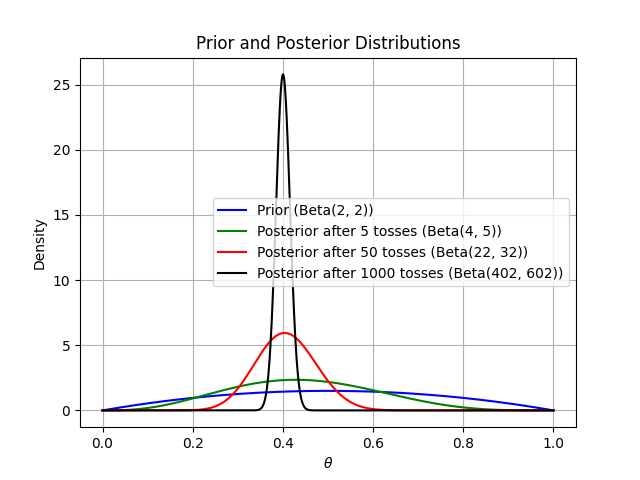
\includegraphics[width=1.0\linewidth]{pdf function of the prior Beta (2,2) and the three posterior distributions.png}
    \caption{Previous three cases and after 1,000 coin tosses}
    \label{fig:enter-label}
\end{figure}
\\
As can be seen above, the posterior distribution after 1000 tosses shrinks at $\theta = 0.4$. If more and more coin tosses, the expected graph will show much closer and narrow at $\theta = 0.4$.  
\\}
\end{enumerate}

\item \textbf{Perceptron. [3pt]} Assume a data set consists only of a single data point $\{(x,+1)\}$. How many times would the Perceptron algorithm mis-classify this point $\x$ before convergence? What if the initial weight vector $\w_0$ was initialized randomly and not as the all-zero vector? Derive the number of times as a function of $\w_0$ and $\x$.

\begin{enumerate}
\item (1 pts) Case 1: $\w_0 = 0$. 

\answer{
\\
If the $x$ is equal to zero, the Perceptron algorithm will mis-classify continuously and even not be converged, satisfying $y(w^{T}x)\leq 0$. On the other hand, $x$ is not equal to zero, for example, $x=1$, The prediction of perceptron is based on the $w^{T}x$, and the weight vector $w_0=0$ causes $w^{T}x=0$. Due to this, at the first iteration, the prediction will mis-classify the point $x$. When the point $(x, +1)$ is mis-classified, the perceptron will update the weight vector:
\[ w_1 = w_0 + x = x\] \\ 
The next iteration of the perceptron use the updated weight vector above to converge:
\[ w_1^{T}x = x^{T}x = ||x||^{2} > 0\]
This means that the perceptron algorithm converges after the first update. \\
Thus, in this case, the perceptron mis-classifies the point one time before converging.
\\}

\item (2 pts) Case 2: $\w_0 !=0$: 

\answer{
\\
When the weight vector $w_0 \ !=0$, we get:
\[ w_0^Tx\]
From the term above, we need to check two cases: \\ 
\[w_0^Tx>0 \ and \ w_0^Tx \leq 0\]
The left case means the point is already correctly classified, and the perceptron will not mis-classify it. The right case means that the point is mis-classified, and the perceptron will use it to update. In the correct classified case, the perceptron does not update the weights, converging immediately. \\

On the other hand, if mis-classified case, $w_0^Tx \leq 0$, the weight vector is updated:
\[ w_1 = w_0 + x\] \\
Then, the new weight vector $w_1$ can be used to check whether the point is now correctly classified or not. So, 
\[ w_1^{T}x = (w_0+x)^Tx = w_0^Tx +||x||^2\] \\
The second term, $||x||^2$, makes $w_1^{T}x$ positive if $(w_0+x)^Tx \leq 0$, leading to correct classification. \\
Thus, we conclude the results above: \\
\[ if w_0^Tx > 0, \text{it would be} \ \text{no misclassification}\]
\[ if w_0^Tx \leq 0, \text{it would be} \ 1 \ \text{misclassification}\]
}
\end{enumerate}

\item \textbf{Bonus: MLE for multi-class logistic regression. [6 pts]} Consider the maximum likelihood estimation problem for multi-class logistic regression using the soft-max function defined below:
\[p(y=k|\mathbf{x}) = \frac{\exp(\mathbf{w}_k^T\mathbf{x})}{\sum_{j=1}^K \exp(\mathbf{w}_j^T\mathbf{x})}\]

We can write out the likelihood function as:
\[ L({\mb w})=\prod_{i=1}^N\prod_{k=1}^K p(y=k|{\mb x}_i)^{y_{ik}}\] where $y_{ik}$ is an indicator variable taking value 1 if $y_i=k$.
\begin{enumerate}
\item (1 pts) Provide the log-likelihood function.\\
\answer{
\\
\[ logL(w) = log\left(\prod_{i=1}^N\prod_{k=1}^K p(y=k|{\mb x}_i)^{y_{ik}}\right)\]
\[ = \sum_{i=1}^{N}log\left(\prod_{k=1}^K p(y=k|{\mb x}_i)^{y_{ik}}\right)\]
\[ = \sum_{i=1}^{N}\sum_{k=1}^{K}y_{ik}log \ p(y=k|{\mb x}_i)\]
\[ = \sum_{i=1}^{N}\sum_{k=1}^{K}y_{ik}log \left(\frac{exp(w_{k}^Tx_i)}{\sum_{j=1}^{K}exp(w_{j}^Tx_i)}\right)\]
\[ = \sum_{i=1}^{N}\sum_{k=1}^{K}y_{ik}\left(log \ exp(w_{k}^Tx_i) - log \sum_{j=1}^{K}exp(w_{j}^Tx_i)\right)\]
\[ = \sum_{i=1}^{N}\sum_{k=1}^{K}y_{ik}\left(w_{k}^{T}x_i-log \left(\sum_{j=1}^{K}exp(w_{j}^Tx_i)\right)\right)\]
\\}

\item (5 pts) Derive the gradient of the log-likelihood function w.r.t the weight vector ${\mb w}_c$ of class $c$.  [Hint: the solution to this problem is provided in the Logistic regression lecture slide. You just need to fill in the missing derivation. Note that for any example $\x_i$, the denominator in the softmax function $\sum_j \exp(\w_j^T\x_i)$ is the same for all $k$--- denoting it as $z_i$ makes it simpler to work through the derivation, but be sure to remember that $z_i$ is a function of all $\w_k$'s.]
\answer{
\\
\\
We use the result above:
\[ \sum_{i=1}^{N}\sum_{k=1}^{K}y_{ik}\left(w_{k}^{T}x_i-log \left(\sum_{j=1}^{K}exp(w_{j}^Tx_i)\right)\right) \]
\[ = \sum_{i=1}^{N}\sum_{k=1}^{K}y_{ik}w_{k}^{T}x_i - \sum_{i=1}^{N}\sum_{k=1}^{K}y_{ik}log \left(\sum_{j=1}^{K}exp(w_{j}^Tx_i)\right) \] \\ 
Differentiate two terms above respectively. Let's start the first term: \\
\[ \frac{\partial}{\partial w_c} \sum_{i=1}^{N}\sum_{k=1}^{K}y_{ik}w_{k}^{T}x_i = \sum_{i=1}^{N}y_{ic}x_i\] \\
The second term is: \\
\[ \frac{\partial}{\partial w_c} \sum_{i=1}^{N}\sum_{k=1}^{K}y_{ik}log \left(\sum_{j=1}^{K}exp(w_{j}^Tx_i)\right)\] \\ 
we utilize $z_i$ to make the mathematical expression above much simpler for derivation.
\[ z_i = \sum_{j=1}^{K}exp(w_{j}^Tx_i)\]
So, we get \\
\[ \Rightarrow \frac{\partial}{\partial w_c} \sum_{i=1}^{N}\sum_{k=1}^{K}y_{ik}log \left(z_i\right) \] \\
The term $y_ik$ can be ignored since it is not dependent on the weight $w$, a constant. The term can be simplified and applied by $z_i$: \\
\[ \frac{\partial}{\partial w_c} \sum_{i=1}^{N}log \left(z_i\right) = \sum_{i=1}^{N} \frac{1}{z_i} \frac{\partial z_i}{\partial w_c} = \sum_{i=1}^{N} \frac{1}{z_i} \frac{\partial}{\partial w_c} \left(\sum_{j=1}^{K}exp(w_{j}^Tx_i)\right)\] \\
Then, we get: \\
\[ \sum_{i=1}^{N} \frac{1}{z_i} exp(w_{c}^{T}x_i)x_i = \sum_{i=1}^{N} \frac{exp(w_{c}^{T}x_i)}{\sum_{j=1}^{K}exp(w_{j}^Tx_i)}x_i = \sum_{i=1}^{N} p(y=c|x_i)x_i\] \\
Thus, we finally obtain: \\
\[ \sum_{i=1}^{N}y_{ic}x_i - \sum_{i=1}^{N} p(y=c|x_i)x_i\]
\[ = \sum_{i=1}^{N} \left(y_{ic} - p(y=c|x_i)\right)x_i\]
}

\end{enumerate}


%
\end{enumerate}

\end{document}
